\documentclass[aspectratio=169,9pt]{beamer}

\usetheme{metropolis}
\usepackage{fontspec}
\setsansfont{DejaVu Sans}
\usepackage{amsmath,amssymb,bm}
\usepackage{booktabs}
\usepackage{tikz}
\usepackage{tikz-3dplot}
\usetikzlibrary{
  arrows.meta, positioning, shapes.geometric, fit, backgrounds,
  calc, decorations.pathreplacing, decorations.markings, patterns, 3d
}
\usepackage{pgfplots}
\pgfplotsset{compat=1.18}
\usepackage{xcolor}
\usepackage{graphicx}
\usepackage{mathtools}
\usepackage{mdframed}
\usepackage{array}
\usepackage{pifont}
\usepackage{listings}
\usepackage{fontawesome5}
\usepackage[numbers,compress]{natbib}
\renewcommand{\bibfont}{\tiny}
\newcommand{\cmark}{\ding{51}}
\newcommand{\xmark}{\ding{55}}

%% ─── Color Palette: "Music Bright" ─────────────────────────────────
\definecolor{mprimary}{HTML}{6C3FC0}   % Violet sáng hơn
\definecolor{maccent}{HTML}{FF9F1C}    % Amber ấm
\definecolor{mgood}{HTML}{2EC4B6}      % Teal sáng
\definecolor{mbad}{HTML}{E5484D}       % Coral (giữ)
\definecolor{mgray}{HTML}{8E8E9A}      % Neutral gray
\definecolor{mdark}{HTML}{2D2640}      % Aubergine nhạt hơn
\definecolor{mlight}{HTML}{F5F0FF}     % Lavender nhạt — nền frametitle MỚI
\definecolor{mlightgold}{HTML}{FFF4E0}
\definecolor{mlightsage}{HTML}{E6F8F5}
\definecolor{mlightred}{HTML}{FDE8E8}

\setbeamercolor{frametitle}{bg=mlight, fg=mprimary}
\setbeamercolor{progress bar}{fg=mprimary}
\setbeamercolor{structure}{fg=mprimary}
\setbeamercolor{title separator}{fg=maccent}

%% ─── mdframed Box Styles ─────────────────────────────────────────────────────
\newmdenv[
  topline=false, bottomline=false, rightline=false,
  linewidth=3pt, linecolor=mprimary!60,
  innerleftmargin=10pt, innerrightmargin=6pt,
  innertopmargin=5pt, innerbottommargin=5pt,
  backgroundcolor=mlight
]{primarybox}

\newmdenv[
  topline=false, bottomline=false, rightline=false,
  linewidth=3pt, linecolor=mgood!70,
  innerleftmargin=10pt, innerrightmargin=6pt,
  innertopmargin=5pt, innerbottommargin=5pt,
  backgroundcolor=mlightsage
]{goodbox}

\newmdenv[
  topline=false, bottomline=false, rightline=false,
  linewidth=3pt, linecolor=mbad!70,
  innerleftmargin=10pt, innerrightmargin=6pt,
  innertopmargin=5pt, innerbottommargin=5pt,
  backgroundcolor=mlightred
]{badbox}

\newmdenv[
  topline=false, bottomline=false, rightline=false,
  linewidth=3pt, linecolor=maccent!80,
  innerleftmargin=10pt, innerrightmargin=6pt,
  innertopmargin=5pt, innerbottommargin=5pt,
  backgroundcolor=mlightgold
]{accentbox}

%% ─── Takeaway Banner ─────────────────────────────────────────────────────────
\newcommand{\takeaway}[1]{%
  \vfill
  \begin{mdframed}[
    linecolor=maccent, linewidth=1.5pt,
    backgroundcolor=mlightgold,
    innertopmargin=5pt, innerbottommargin=5pt,
    innerleftmargin=10pt, innerrightmargin=10pt,
    roundcorner=3pt, skipabove=4pt, skipbelow=0pt
  ]
  \centering\small\bfseries\color{mprimary} #1
  \end{mdframed}%
}

%% ─── Image placeholder (thay bằng screenshot thật sau) ───────────────
\newcommand{\imgplaceholder}[2][0.9\textwidth]{%
  \begin{tikzpicture}
    \node[draw=mprimary!50, fill=mlight, rounded corners=4pt,
          dashed, line width=1pt, minimum width=#1, minimum height=0.58\textheight,
          align=center, font=\footnotesize\color{mprimary!80}] {%
      \faImage~\textbf{[ẢNH CẦN CHÈN]}\\[4pt]#2};
  \end{tikzpicture}%
}

\newcommand{\eqbars}[1]{%
  \begin{tikzpicture}[baseline]
    \foreach \h in {0.18,0.42,0.28,0.55,0.34,0.48,0.22}{
      \fill[#1] (0,0) rectangle (0.12,\h); \pgftransformxshift{6mm}}
  \end{tikzpicture}}

%% ─── TikZ styles ─────────────────────────────────────────────────────────────
\tikzset{
  pbox/.style={draw=mprimary!50, fill=mlight, rounded corners=3pt,
               minimum height=0.65cm, font=\small, inner sep=5pt},
  gbox/.style={draw=mgood!60, fill=mlightsage, rounded corners=3pt,
               minimum height=0.65cm, font=\small, inner sep=5pt},
  rbox/.style={draw=mbad!60, fill=mlightred, rounded corners=3pt,
               minimum height=0.65cm, font=\small, inner sep=5pt},
  abox/.style={draw=maccent!70, fill=mlightgold, rounded corners=3pt,
               minimum height=0.65cm, font=\small, inner sep=5pt},
  darkbox/.style={draw=mprimary, fill=mprimary!85, text=white, rounded corners=3pt,
                  minimum height=0.7cm, font=\small\bfseries, inner sep=6pt},
  arr/.style={->, thick, mprimary},
  darr/.style={->, dashed, thin, mgray},
  srcbox/.style={draw=maccent!70, fill=mlightgold, rounded corners=3pt,
                 minimum height=0.62cm, font=\scriptsize, inner sep=4pt},
  aibox/.style={draw=maccent, fill=maccent!90, text=white, rounded corners=4pt,
                minimum height=0.7cm, font=\small\bfseries, inner sep=6pt},
}

%% ─── Title ───────────────────────────────────────────────────────────────────
\title{\textbf{World Music Intelligence Monitor}}
\subtitle{Phân tích \& cập nhật bản tin âm nhạc toàn cầu theo thời gian thực}
\author{Nhóm SonicT2All --- Phân tích Dữ liệu Thông minh}
\date{}

\begin{document}

% ─── Slide 0: Title ─────────────────────────────────────────────────────────
\begin{frame}[plain]
\vspace{0.4cm}
\begin{columns}[c]
\column{0.52\textwidth}
  \begin{center}
    {\Huge\bfseries\color{mprimary} World Music\\[4pt] Intelligence Monitor}\\[10pt]
    {\large\itshape\color{mprimary!80} Phân tích \& cập nhật bản tin âm nhạc toàn cầu — realtime}\\[14pt]
    {\large\bfseries SonicT2All}\\[4pt]
    {\small\color{mgray} Phân tích Dữ liệu Thông minh}\\[8pt]
    {\scriptsize\color{mgray} 
      GVHD: TS. Nguyễn Tiến Huy, ThS. Nguyễn Thanh Tình\\[3pt]
      Thành viên: Bàng Mỹ Linh, Lại Nguyễn Hồng Thanh,\\
      Phan Huỳnh Châu Thịnh, Nguyễn Gia Bảo, Nguyễn Ngọc Như Quỳnh
    }\\[12pt]
    \eqbars{maccent}
  \end{center}

\column{0.48\textwidth}
  \begin{center}
    \begin{tikzpicture}[every node/.style={font=\scriptsize}]
      \node[aibox, circle, minimum size=1.8cm, align=center, inner sep=0pt] (center) at (0,0) {\faChartLine\\[2pt]Monitor};
      
      \node[srcbox] (s1) at (90:2.1cm) {Last.fm};
      \node[srcbox] (s2) at (18:2.1cm) {\faYoutube~YouTube};
      \node[srcbox] (s3) at (162:2.1cm) {\faSpotify~Spotify};
      \node[srcbox] (s4) at (306:2.1cm) {\faReddit~Reddit};
      \node[srcbox] (s5) at (234:2.1cm) {Deezer};
      
      \draw[arr] (s1) -- (center);
      \draw[arr] (s2) -- (center);
      \draw[arr] (s3) -- (center);
      \draw[arr] (s4) -- (center);
      \draw[arr] (s5) -- (center);
      
      \node[pbox, font=\scriptsize, inner sep=3pt] (o1) at (205:2.6cm) {Dashboard};
      \node[pbox, font=\scriptsize, inner sep=3pt] (o2) at (270:2.6cm) {World Map};
      \node[pbox, font=\scriptsize, inner sep=3pt] (o3) at (335:2.6cm) {AI Chat};
      
      \draw[darr] (center) -- (o1);
      \draw[darr] (center) -- (o2);
      \draw[darr] (center) -- (o3);
      
    \end{tikzpicture}
  \end{center}
\end{columns}
\end{frame}

% ─── Slide 1: Outline ────────────────────────────────────────────────────────
\begin{frame}{Lộ Trình Trình Bày}
\vspace{0.8cm}
\begin{center}
\begin{tikzpicture}[x=2.5cm, y=1cm]
  \tikzstyle{stepbox} = [fill=white, rounded corners=6pt, text width=2.1cm, align=center, inner sep=4pt, minimum height=1.4cm, line width=1pt]
  \tikzstyle{stepnum} = [circle, text=white, font=\footnotesize\bfseries, inner sep=0pt, minimum size=0.6cm]
  
  %% Connecting Line
  \draw[line width=1.5pt, mprimary!20] (0, 1.2) -- (4, 1.2);

  %% Step 1
  \node[stepbox, draw=mprimary] (b1) at (0, -0.2) {\textbf{\color{mprimary}TỔNG QUAN}\\[3pt]\scriptsize Kiến trúc \&\\data pipeline};
  \node[stepnum, fill=mprimary] (n1) at (0, 1.2) {1};
  \draw[thick, mprimary] (n1) -- (b1);

  %% Step 2
  \node[stepbox, draw=mprimary] (b2) at (1, -0.2) {\textbf{\color{mprimary}TRỰC QUAN HÓA}\\[3pt]\scriptsize Dashboard \&\\cảm xúc};
  \node[stepnum, fill=mprimary] (n2) at (1, 1.2) {2};
  \draw[thick, mprimary] (n2) -- (b2);

  %% Step 3
  \node[stepbox, draw=maccent, line width=1.4pt] (b3) at (2, -0.2) {\textbf{\color{maccent}PHÂN TÍCH}\\[3pt]\scriptsize Phân cụm \&\\phát hiện viral \faStar};
  \node[stepnum, fill=maccent] (n3) at (2, 1.2) {3};
  \draw[thick, maccent] (n3) -- (b3);

  %% Step 4
  \node[stepbox, draw=maccent] (b4) at (3, -0.2) {\textbf{\color{maccent}DỰ ĐOÁN}\\[3pt]\scriptsize XGBoost \&\\AI Agent};
  \node[stepnum, fill=maccent] (n4) at (3, 1.2) {4};
  \draw[thick, maccent] (n4) -- (b4);

  %% Step 5
  \node[stepbox, draw=mgood] (b5) at (4, -0.2) {\textbf{\color{mgood}ĐÁNH GIÁ}\\[3pt]\scriptsize Điểm mạnh \&\\hướng phát triển};
  \node[stepnum, fill=mgood] (n5) at (4, 1.2) {5};
  \draw[thick, mgood] (n5) -- (b5);

\end{tikzpicture}
\end{center}

\vspace{0.8cm}
\begin{accentbox}
\centering\small\itshape
Từ dữ liệu thô đa nền tảng $\to$ bản tin âm nhạc thông minh, realtime.
\end{accentbox}
\end{frame}

% ─── SECTION DIVIDER ──────────────────────────────────────────────────────────
\section{TỔNG QUAN \& KIẾN TRÚC}

% ─── Slide 2: Bài Toán & Giải Pháp ───────────────────────────────────────────
\begin{frame}{Tổng Quan Nền Tảng}

\begin{columns}[T]
\column{0.5\textwidth}
\vspace{0.4cm}
\begin{itemize}\footnotesize\setlength\itemsep{10pt}
  \item \textbf{Global Music Intelligence:} Phân tích dữ liệu âm nhạc theo thời gian thực.
  \item \textbf{Hệ sinh thái đa tính năng:} Từ Giám sát tổng quan (Dashboard), Phân cụm thị hiếu (World Map), đến Dự đoán (Prediction).
  \item \textbf{Đa nguồn dữ liệu:} Tích hợp luồng dữ liệu từ YouTube, Spotify, Last.fm và mạng xã hội Reddit.
  \item \textbf{Tích hợp AI Đích thực:} Tiên phong ứng dụng mô hình ngôn ngữ lớn (Gemini) vào hệ thống phân tích.
\end{itemize}

\column{0.46\textwidth}
\begin{center}
  \begin{tikzpicture}
    \node[draw=mprimary!50, fill=white, rounded corners=4pt, dashed, line width=1pt, minimum width=\linewidth, minimum height=0.3\textheight, align=center, font=\footnotesize\color{mprimary!80}] {%
      \faImage~\textbf{[ẢNH CẦN CHÈN]}\\[4pt]Bright Mode\\\% [IMG] overview-bright.png};
  \end{tikzpicture}
  
  \vspace{0.15cm}
  \begin{tikzpicture}
    \node[draw=mprimary!50, fill=mdark, rounded corners=4pt, dashed, line width=1pt, minimum width=\linewidth, minimum height=0.3\textheight, align=center, font=\footnotesize\color{mlight}] {%
      \faImage~\textbf{[ẢNH CẦN CHÈN]}\\[4pt]Dark Mode\\\% [IMG] overview-dark.png};
  \end{tikzpicture}
\end{center}
\end{columns}

\takeaway{Nền tảng phân tích âm nhạc đa nguồn, đa tính năng, dẫn dắt bởi AI.}

\end{frame}

% ─── Slide 3: Kiến Trúc Hệ Thống ─────────────────────────────────────────────
\begin{frame}{Kiến Trúc Hệ Thống}

\begin{center}
\resizebox{0.9\textwidth}{!}{
\begin{tikzpicture}[every node/.style={font=\scriptsize}, x=1.9cm, y=1.2cm]

  % Layer 1: FRONTEND
  \node[pbox, minimum width=16.5cm, minimum height=1.3cm, fill=mprimary!10, draw=mprimary!40, align=left] (fe) at (0, 2.2) {};
  \node[font=\bfseries\color{mprimary}, anchor=north west, xshift=4pt, yshift=-4pt] at (fe.north west) {FRONTEND \textmd{\scriptsize(Next.js 14 $\cdot$ App Router $\cdot$ TypeScript)}};
  
  \node[pbox, fill=white, minimum height=0.4cm] (d1) at (-2.5, 1.9) {Dashboard};
  \node[pbox, fill=white, minimum height=0.4cm] (d2) at (0, 1.9) {World Map};
  \node[pbox, fill=white, minimum height=0.4cm] (d3) at (2.5, 1.9) {AI Chat};
  \node[font=\scriptsize\color{mgray}, anchor=north east, xshift=-4pt, yshift=-4pt] at (fe.north east) {Vercel $\cdot$ port 3000};

  % Layer 2: BACKEND
  \node[darkbox, minimum width=16.5cm, minimum height=1.3cm, align=left] (be) at (0, 0.6) {};
  \node[font=\bfseries\color{white}, anchor=north west, xshift=4pt, yshift=-4pt] at (be.north west) {BACKEND \textmd{\scriptsize(FastAPI $\cdot$ Python 3.11 $\cdot$ Uvicorn)}};
  
  \node[pbox, fill=white, text=mprimary, minimum height=0.4cm] (b1) at (-3.2, 0.3) {Routers};
  \node[pbox, fill=white, text=mprimary, minimum height=0.4cm] (b2) at (-1.1, 0.3) {Services};
  \node[pbox, fill=white, text=mprimary, minimum height=0.4cm] (b3) at (1.1, 0.3) {AI/ML};
  \node[pbox, fill=white, text=mprimary, minimum height=0.4cm] (b4) at (3.2, 0.3) {Scheduler};
  \node[font=\scriptsize\color{white}, anchor=north east, xshift=-4pt, yshift=-4pt] at (be.north east) {Render.com $\cdot$ port 8000};

  % Layer 3: AI / EXTERNAL
  \node[draw=mgray!50, dashed, rounded corners=3pt, minimum width=7.2cm, minimum height=1.8cm] (ext_left) at (-2.4, -1.55) {};
  \node[font=\scriptsize\color{mgray}, anchor=south west, xshift=4pt, yshift=2pt] at (ext_left.north west) {External Sources};
  
  \node[srcbox] (s1) at (-3.7, -1.2) {Last.fm};
  \node[srcbox] (s2) at (-2.4, -1.2) {\faYoutube};
  \node[srcbox] (s3) at (-1.1, -1.2) {\faReddit};
  \node[srcbox] (s4) at (-3.0, -1.9) {Deezer};
  \node[srcbox] (s5) at (-1.8, -1.9) {\faSpotify};

  \node[draw=mgray!50, dashed, rounded corners=3pt, minimum width=7.5cm, minimum height=1.8cm] (ext_right) at (2.4, -1.55) {};
  \node[font=\scriptsize\color{mgray}, anchor=south east, xshift=-4pt, yshift=2pt] at (ext_right.north east) {AI Models};
  
  \node[aibox] (a1) at (1.1, -1.2) {Gemini};
  \node[aibox] (a2) at (3.3, -1.2) {K-Means / XGBoost};
  \node[aibox] (a3) at (2.4, -1.9) {ReAct Agent};

  % Layer 4: DATA LAYER
  \node[pbox, minimum width=16.5cm, minimum height=1.2cm, fill=mprimary!10, draw=mprimary!40, align=left] (db) at (0, -3.1) {};
  \node[font=\bfseries\color{mprimary}, anchor=north west, xshift=4pt, yshift=-4pt] at (db.north west) {DATA LAYER};
  
  \node[pbox, fill=white, minimum height=0.4cm] (db1) at (-2.8, -3.3) {Firebase Firestore};
  \node[pbox, fill=white, minimum height=0.4cm] (db2) at (0, -3.3) {map\_cache.json};
  \node[pbox, fill=white, minimum height=0.4cm] (db3) at (2.8, -3.3) {In-memory cache};

  % Arrows
  \draw[<->, thick, mprimary] (fe.south) -- (be.north) node[midway, right, font=\scriptsize] {HTTP REST + SSE};
  
  \draw[<->, thick, mprimary] (be.south -| ext_left.north) -- (ext_left.north) node[midway, left, font=\scriptsize, fill=white, inner sep=2pt] {HTTP calls};
  \draw[<->, thick, mprimary] (be.south -| ext_right.north) -- (ext_right.north) node[midway, right, font=\scriptsize, fill=white, inner sep=2pt] {HTTP calls};
  
  \draw[<->, thick, mprimary] (be.south) -- (db.north) node[midway, right, font=\scriptsize, fill=white, inner sep=2pt] {Cache IO};

\end{tikzpicture}
}
\end{center}

\vspace{-0.2cm}
\begin{center}
  \tiny\itshape\color{mgray} Kiến trúc 3-tier + lớp AI — mỗi tầng deploy độc lập.
\end{center}

\takeaway{3 tầng tách biệt + lớp AI — dữ liệu chảy một chiều, dễ mở rộng.}

\end{frame}

% ─── Slide 4: Data Pipeline ──────────────────────────────────────────────────
\begin{frame}{Data Pipeline: Đa Nguồn \& Realtime}

\begin{center}
\begin{tikzpicture}[every node/.style={font=\small}, x=2.5cm, y=0.6cm]
  % Sources
  \node[srcbox, minimum width=2cm] (s1) at (0, 2) {Last.fm};
  \node[srcbox, minimum width=2cm] (s2) at (0, 1) {\faYoutube~YouTube};
  \node[srcbox, minimum width=2cm] (s3) at (0, 0) {\faReddit~Reddit};
  \node[srcbox, minimum width=2cm] (s4) at (0, -1) {Deezer};
  \node[srcbox, minimum width=2cm] (s5) at (0, -2) {\faSpotify~Spotify};
  
  \node[font=\tiny\color{mgray}, below=2pt of s5] {miễn phí, không cần key};

  % Scheduler
  \node[darkbox, align=center] (sched) at (1.8, 0) {Scheduler\\(APScheduler)};

  % Cache
  \node[draw=mgray!50, dashed, rounded corners=3pt, minimum width=3.2cm, minimum height=2.2cm] (cache_bg) at (3.5, -0.15) {};
  \node[font=\scriptsize\color{mgray}, anchor=south, yshift=2pt] at (cache_bg.north) {Cache Layer};

  \node[pbox, minimum width=2.5cm] (fs) at (3.5, 0.4) {Firebase Firestore};
  \node[pbox, minimum width=2.5cm] (mc) at (3.5, -0.7) {map\_cache.json};

  % Arrows
  \draw[arr] (s1.east) to[out=0, in=180] node[pos=0.45, above, sloped, font=\scriptsize, fill=white, inner sep=1pt] {poll 6h} (sched.west);
  
  \draw [decorate, decoration={brace, amplitude=4pt}, thick, mgray] 
    ([xshift=4pt, yshift=2pt]s2.north east) -- ([xshift=4pt, yshift=-2pt]s5.south east) 
    node [midway, right=4pt, font=\scriptsize\color{mgray}] (brace_node) {on-demand};

  \draw[arr] (brace_node.east) to[out=0, in=180] (sched.west);

  \draw[arr] (sched.east) -- (cache_bg.west);
  
  \node[pbox] (router) at (1.8, 2.4) {Router $\to$ JSON};
  \draw[arr, rounded corners] (cache_bg.north) |- (router.east);
  
\end{tikzpicture}
\end{center}

\vspace{0.1cm}
\begin{itemize}\footnotesize\setlength\itemsep{3pt}
  \item Polling 6h cho Last.fm — tối ưu quota Firebase free tier.
  \item 4 nguồn còn lại fetch on-demand, song song bằng \texttt{asyncio.gather}.
  \item Cache 3 lớp: Firestore (cloud) $\cdot$ file JSON $\cdot$ in-memory.
\end{itemize}

\vspace{0.1cm}
\begin{primarybox}
  \textbf{Vì sao polling, không webhook?}\\[2pt]
  \footnotesize
  Các nền tảng nhạc không cung cấp webhook — polling + cache là lựa chọn thực tế.
\end{primarybox}

\takeaway{5+ nguồn, polling 6h + on-demand, cache 3 lớp — luôn có dữ liệu để hiển thị.}

\end{frame}

% ─── Slide 5: Bảo Mật & Định Danh ────────────────────────────────────────────
\begin{frame}{Bảo Mật \& Định Danh}

\begin{columns}[T]
\column{0.5\textwidth}
\begin{center}
\begin{tikzpicture}[every node/.style={font=\footnotesize}, y=-1.0cm, scale=0.7, transform shape]
  \node[pbox] (user) at (0, 0) {Người dùng};
  
  \node[darkbox] (clerk) at (0, 1.1) {Clerk Middleware};
  
  \node[draw=mgray, dashed, rounded corners=3pt, minimum width=3.2cm, minimum height=0.6cm] (pub) at (-1.8, 2.3) {Route public};
  \node[draw=mgray, dashed, rounded corners=3pt, minimum width=3.2cm, minimum height=0.6cm] (prot) at (2.0, 2.3) {Route protected};
  
  \node[font=\tiny\color{mgray}, below=2pt of pub] {/, /sign-in};
  
  \node[gbox] (pass) at (-1.8, 3.4) {Cho qua};
  \node[darkbox] (auth) at (2.0, 3.4) {auth().protect()};
  
  \node[gbox] (dash) at (2.0, 4.5) {Vào Dashboard};
  
  \node[font=\scriptsize\color{mgray}, align=center] (login) at (4.2, 3.4) {Sign-in\\(chưa login)};
  
  \draw[arr] (user) -- (clerk);
  \draw[arr] (clerk) -- (pub.north);
  \draw[arr] (clerk) -- (prot.north);
  \draw[arr] (pub) -- (pass);
  \draw[arr] (prot) -- (auth);
  \draw[arr] (auth) -- (dash);
  
  \draw[darr] (auth) -- (login);
\end{tikzpicture}
\end{center}

\column{0.48\textwidth}
\vspace{0.3cm}

\begin{primarybox}
  \textbf{Clerk — Identity Platform}\\[4pt]
  \footnotesize
  \faCheck~ SSO: đăng nhập qua Google / Email-Password.\\[4pt]
  \faCheck~ Quản lý session, connected accounts minh bạch.
\end{primarybox}

\vspace{0.4cm}
\begin{goodbox}
  \textbf{Bảo vệ được gì}\\[4pt]
  \footnotesize
  \faLock~ Chặn truy cập trái phép vào Data Pipeline \& AI Chat.\\[4pt]
  \faLock~ Nền móng sẵn sàng cho RBAC (Admin / Viewer).
\end{goodbox}

\end{columns}

\takeaway{Clerk lo định danh \& phân quyền — nhóm tập trung vào phần phân tích.}

\end{frame}

% ─── Slide 6: Hồ Sơ Cá Nhân ──────────────────────────────────────────────────
\begin{frame}{Hồ Sơ Cá Nhân}

\begin{columns}[T]
\column{0.48\textwidth}
\begin{center}
  \imgplaceholder[\linewidth]{Trang User Management\\\% [IMG] profile-page.png}
\end{center}

\column{0.48\textwidth}
\vspace{0.6cm}
\begin{itemize}\footnotesize\setlength\itemsep{12pt}
  \item \textbf{Quản trị hồ sơ toàn diện:}\\ Tích hợp Portal quản lý tài khoản trực quan cho End-user.
  \item \textbf{Định danh liên kết (Connected Accounts):}\\ Kiểm soát và đồng bộ hóa luồng đăng nhập SSO (Google, Github) một cách minh bạch, an toàn.
  \item \textbf{Mở rộng phân quyền (Future-proof RBAC):}\\ Nền móng CSDL người dùng sẵn sàng triển khai phân quyền theo vai trò (Admin / Viewer).
\end{itemize}
\end{columns}

\takeaway{Nền móng người dùng sẵn sàng mở rộng — từ đăng nhập đến phân quyền.}

\end{frame}

% ─── SECTION DIVIDER ──────────────────────────────────────────────────────────
\section{THU THẬP \& TRỰC QUAN HÓA}

% ─── Slide 6: Dashboard ──────────────────────────────────────────────────────
\begin{frame}{Dashboard: Giám Sát Tổng Quan}

\begin{columns}[T]
\column{0.58\textwidth}
  % [IMG] dashboard-fullpage.png — chụp full trang /dashboard ở light mode
  \imgplaceholder[0.96\linewidth]{Trang /dashboard — Global Top 50 + MIS + AI Briefing}

\column{0.4\textwidth}
  \vspace{0.2cm}
  \begin{itemize}\footnotesize\setlength\itemsep{8pt}
    \item[\faBell] Live Anomaly Alert — phát hiện spike realtime.
    \item[\faChartBar] Global Top 50 kèm điểm MIS.
  \end{itemize}
  
  \vspace{-0.1cm}
  \begin{accentbox}
    \footnotesize MIS = Plays + Listeners + trọng số xu hướng.
  \end{accentbox}
  \vspace{0.1cm}
  
  \begin{itemize}\footnotesize\setlength\itemsep{8pt}
    \item[\faFilter] Bộ lọc động: Today / This Week / This Month.
    \item[\faThLarge] Unified UI — số liệu thô + AI Briefing trên 1 màn hình.
  \end{itemize}
\end{columns}

\takeaway{Một màn hình — số liệu realtime và bản tin AI cạnh nhau.}

\end{frame}

% ─── Slide 7: Daily Briefing & Phân Tích Cảm Xúc ─────────────────────────────
\begin{frame}{Daily Briefing \& Phân Tích Cảm Xúc}

\begin{center}
\begin{tikzpicture}[every node/.style={font=\small}, x=2.0cm, y=1.2cm]
  \node[srcbox] (s1) at (0, 1) {Last.fm Top Charts};
  \node[srcbox] (s2) at (0, 0) {Reddit Posts};
  \node[srcbox] (s3) at (0, -1) {Deezer TikTok};
  
  \node[aibox, align=center] (vader) at (1.4, 0) {VADER NLP};
  \node[font=\tiny\color{mgray}, below=2pt of vader] {Neg / Neu / Pos};
  
  \node[pbox] (json) at (2.8, 0) {JSON tổng hợp};
  
  \node[aibox, minimum height=0.8cm, align=center] (gemini) at (4.3, 0) {Gemini 3.1\\Flash-Lite};
  
  \node[gbox, align=center] (out) at (5.7, 0) {Bản tin\\có cấu trúc};
  
  \draw[arr] (s2) -- (vader);
  \draw[arr] (vader) -- (json);
  \draw[arr] (s1.east) -- (json.west);
  \draw[arr] (s3.east) -- (json.west);
  \draw[arr] (json) -- (gemini);
  \draw[arr] (gemini) -- (out);
\end{tikzpicture}
\end{center}

\vspace{0.4cm}
\begin{columns}[T]
\column{0.48\textwidth}
\begin{primarybox}
  \textbf{Đầu vào}\\[4pt]
  \footnotesize
  Top Charts + Reddit mentions + điểm sentiment $\to$ đóng gói JSON.
\end{primarybox}

\column{0.48\textwidth}
\begin{goodbox}
  \textbf{Đầu ra (5 mục)}\\[4pt]
  \footnotesize
  Tổng quan $\cdot$ TikTok Viral Alert $\cdot$ Dự báo tuần tới\\[3pt]
  \tiny\color{mgray} \itshape Có fallback khi Gemini hết quota.
\end{goodbox}
\end{columns}

\takeaway{VADER chấm cảm xúc, Gemini viết bản tin — raw data thành insight tự động.}

\end{frame}

% ─── Slide 9: Trực Quan Hóa & Phân Tích ──────────────────────────────────────
\begin{frame}{Trực Quan Hóa \& Phân Tích}

\begin{columns}[T]
\column{0.48\textwidth}
\begin{center}
  \imgplaceholder[\linewidth]{Giao diện trực quan hóa đa nguồn\\\% [IMG] visualization-analysis.png}
\end{center}

\column{0.48\textwidth}
\vspace{0.4cm}
\begin{itemize}\footnotesize\setlength\itemsep{10pt}
  \item \textbf{Multi-source Tracking:}
    \begin{itemize}\scriptsize\setlength\itemsep{4pt}
      \item Last.fm $\to$ Top Tracks \& phân phối thể loại.
      \item YouTube $\to$ Time-series View (6 ngày).
      \item Deezer TikTok $\to$ Viral Ranking Heatmap.
    \end{itemize}
  \item \textbf{Hit Prediction \& Giải Thích Dự Đoán:}\\
    Radar Chart: Growth $\cdot$ Buzz $\cdot$ Sentiment $\cdot$ Viral $\cdot$ Hit Prob.
\end{itemize}
\end{columns}

\takeaway{Gom mọi góc nhìn từ số liệu thô đến dự đoán AI lên cùng một màn hình.}

\end{frame}

% ─── Slide 10: Phân Phối Dữ Liệu ─────────────────────────────────────────────
\begin{frame}{Phân Phối Dữ Liệu}

\begin{columns}[T]
\column{0.55\textwidth}
\begin{center}
  \imgplaceholder[\linewidth]{Biểu đồ phân phối long-tail\\\% [IMG] pareto-distribution.png}
\end{center}

\column{0.43\textwidth}
\vspace{0.4cm}
\begin{itemize}\footnotesize\setlength\itemsep{10pt}
  \item \textbf{Pareto Distribution (Long-tail):}\\ Top 1 chiếm áp đảo $\to$ quy luật 80/20 rõ nét.
  \item \textbf{Cross-platform Tracking:}\\ YouTube Views \& Likes; Reddit r/Music Upvotes \& Comments.
  \item \textbf{Sentiment Bar:}\\ Tích cực (teal) / Tiêu cực (coral) $\to$ Phát hiện sớm khủng hoảng truyền thông.
\end{itemize}
\end{columns}

\takeaway{Dữ liệu nhạc có dạng long-tail — vài bài hút phần lớn lượt nghe.}

\end{frame}

% ─── SECTION DIVIDER ──────────────────────────────────────────────────────────
\section{PHÂN TÍCH THÔNG MINH}

% ─── Slide 11: World Map — Phân Cụm Thị Hiếu (K-Means) ───────────────────────
\begin{frame}{World Map — Phân Cụm K-Means}

\begin{columns}[T]
\column{0.46\textwidth}
  \begin{center}
  \begin{tikzpicture}[every node/.style={font=\scriptsize}, y=-0.9cm]
    \node[srcbox, align=center] (b1) at (0, 0) {Deezer chart + Last.fm tags\\(89 quốc gia)};
    \node[pbox] (b2) at (0, 1.2) {Vector 16 thể loại / quốc gia};
    \node[aibox] (b3) at (0, 2.2) {K-Means (k=6)};
    \node[pbox] (b4) at (0, 3.2) {PCA $\to$ toạ độ 2D};
    \node[gbox] (b5) at (0, 4.2) {Nhãn cụm: POP-dominant…};
    
    \draw[arr] (b1) -- (b2);
    \draw[arr] (b2) -- (b3);
    \draw[arr] (b3) -- (b4);
    \draw[arr] (b4) -- (b5);
  \end{tikzpicture}
  
  \vspace{0.2cm}
  \tiny\color{mgray} \itshape Cache map\_cache.json — lần đầu ~60--90s, sau đó tức thì.
  \end{center}

\column{0.48\textwidth}
  % [IMG] worldmap-page.png — chụp /map có popup 1 quốc gia
  \imgplaceholder[\linewidth]{Trang /map — bản đồ Leaflet tô màu theo cụm}
  
  \vspace{0.1cm}
  \begin{center}
    \tiny\color{mgray} \itshape Click quốc gia $\to$ AI Cultural Insight (Gemini) giải thích nguyên nhân văn hóa.
  \end{center}
\end{columns}

\vspace{0.1cm}
\begin{accentbox}
  \footnotesize Phát hiện dị biệt: Việt Nam rơi vào cụm Latin-dominant — Gemini lý giải.
\end{accentbox}

\takeaway{K-Means gom 89 quốc gia theo gu nhạc — bản đồ kể chuyện văn hóa.}

\end{frame}

% ─── Slide 12: Trending — Phát Hiện Viral ────────────────────────────────────
\begin{frame}{Trending — Phát Hiện Viral}

\begin{columns}[T]
\column{0.5\textwidth}
  \begin{center}
  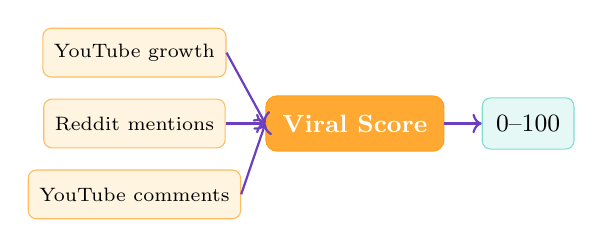
\begin{tikzpicture}[every node/.style={font=\scriptsize}]
    \node[srcbox] (s1) at (0, 0.9) {YouTube growth};
    \node[srcbox] (s2) at (0, 0) {Reddit mentions};
    \node[srcbox] (s3) at (0, -0.9) {YouTube comments};
    
    \node[aibox] (viral) at (2.8, 0) {Viral Score};
    \node[gbox] (out) at (5, 0) {0--100};
    
    \draw[arr] (s1.east) -- (viral.west);
    \draw[arr] (s2.east) -- (viral.west);
    \draw[arr] (s3.east) -- (viral.west);
    \draw[arr] (viral) -- (out);
  \end{tikzpicture}
  \end{center}
  
  \vspace{0.4cm}
  \begin{primarybox}
    \footnotesize Viral = 50\% $\cdot$ YouTube + 30\% $\cdot$ Reddit + 20\% $\cdot$ Comments
  \end{primarybox}

\column{0.48\textwidth}
  \begin{itemize}\footnotesize\setlength\itemsep{8pt}
    \item Z-score trên chuỗi tăng view — phát hiện spike (ngưỡng 2.5).
    \item Isolation Forest — đánh dấu bài bất thường trong batch.
    \item Xếp hạng theo Velocity (vận tốc tăng), không chỉ tổng view.
  \end{itemize}
  
  \vspace{0.2cm}
  \begin{accentbox}
    \footnotesize \faQuestionCircle~ Nút "Tại sao viral?" — Gemini tổng hợp sự kiện / trend TikTok.
  \end{accentbox}
\end{columns}

\takeaway{Z-score + Isolation Forest + Gemini — phát hiện và giải thích viral.}

\end{frame}

% ─── Slide 13: Social Listening ──────────────────────────────────────────────
\begin{frame}{Social Listening}

\begin{columns}[T]
\column{0.55\textwidth}
\begin{center}
  \imgplaceholder[\linewidth]{Trang Social Listening\\\% [IMG] social-listening.png}
\end{center}

\column{0.43\textwidth}
\vspace{0.4cm}
\begin{itemize}\footnotesize\setlength\itemsep{10pt}
  \item \textbf{Multi-subreddit:}\\ Theo dõi r/Music, r/kpop, r/hiphopheads.
  \item \textbf{VADER NLP:}\\ Phân loại Pos / Neu / Neg \& tổng hợp Mentions 24h.
  \item \textbf{Gemini Contextual AI Insight:}\\ 
    \begin{itemize}\scriptsize\setlength\itemsep{4pt}
      \item Chủ đề chính.
      \item Mức độ quan tâm.
      \item Góc nhìn cộng đồng.
      \item Tác động truyền thông.
    \end{itemize}
\end{itemize}
\end{columns}

\takeaway{Đo nhiệt cộng đồng và lấy insight tự động từ hàng ngàn bình luận.}

\end{frame}

% ─── SECTION DIVIDER ──────────────────────────────────────────────────────────
\section{DỰ ĐOÁN \& AI AGENT}

% ─── Slide 14: Dự Đoán Hit ───────────────────────────────────────────────────
\begin{frame}{Dự Đoán Hit}

\begin{columns}[T]
\column{0.55\textwidth}
\begin{center}
  \imgplaceholder[\linewidth]{Form nhập \& Kết quả dự đoán\\\% [IMG] predict-page.png}
\end{center}

\column{0.43\textwidth}
\vspace{0.4cm}
\begin{itemize}\footnotesize\setlength\itemsep{10pt}
  \item \textbf{Model Deployment:}\\ Đưa mô hình XGBoost vào Web App để dự đoán thời gian thực.
  \item \textbf{Feature Pipeline:}\\ Tự động crawl dữ liệu từ Deezer, YouTube, Reddit, Last.fm khi nhập tên bài hát.
  \item \textbf{Dự đoán Xác suất:}\\ Output \% xác suất Hit và phân loại rủi ro (Watch / Low confidence).
  \item \textbf{Tích hợp Đa phương tiện:}\\ Cho phép nghe preview ngay trên Web.
\end{itemize}
\end{columns}

\takeaway{Nhập 1 URL $\to$ quy nạp features $\to$ XGBoost dự đoán Hit/Flop tức thời.}

\end{frame}

% ─── Slide 15: Giải Thích Dự Đoán ────────────────────────────────────────────
\begin{frame}{Giải Thích Dự Đoán}

\begin{columns}[T]
\column{0.55\textwidth}
\begin{center}
  \imgplaceholder[\linewidth]{Radar Chart \& Lời giải thích\\\% [IMG] explain-predict.png}
\end{center}

\column{0.43\textwidth}
\vspace{0.4cm}
\begin{itemize}\footnotesize\setlength\itemsep{10pt}
  \item \textbf{Chuyển hóa kết quả:}\\ Thành các phân tích ngữ nghĩa dễ hiểu cho con người.
  \item \textbf{Radar 5 trục:}\\ Memeability, Emotional Hook, Danceability, Lyrics và Shock Value.
  \item \textbf{AI Phiên dịch:}\\ Gemini đọc trọng số XGBoost để giải thích bằng lời văn: Tại sao đạt mức này?
  \item \textbf{Đề xuất hành động:}\\ Trực tiếp đưa ra tư vấn chiến lược cho người dùng.
\end{itemize}
\end{columns}

\takeaway{AI không chỉ báo số, mà còn chỉ ra nguyên nhân và hướng hành động.}

\end{frame}

% ─── Slide 16: AI Chat ───────────────────────────────────────────────────────
\begin{frame}{AI Chat}

\begin{columns}[T]
\column{0.55\textwidth}
\begin{center}
  \imgplaceholder[\linewidth]{Agent chat \& Thought trace\\\% [IMG] chat-page.png}
\end{center}

\column{0.43\textwidth}
\vspace{0.4cm}
\begin{itemize}\footnotesize\setlength\itemsep{10pt}
  \item \textbf{Reasoning + Acting:}\\ Biến LLM thành Agent suy luận logic và tự gọi Web Search, DB Query.
  \item \textbf{Graceful Error Handling:}\\ Tự chuyển hướng sang Internal Knowledge khi tool gặp lỗi.
  \item \textbf{Truy vấn Tự nhiên:}\\ Tương tác trực tiếp với dữ liệu thị trường bằng ngôn ngữ con người.
\end{itemize}
\end{columns}

\takeaway{Agent tự phân tích, dùng tool, tự sửa lỗi — vượt giới hạn hỏi đáp tĩnh.}

\end{frame}

% ─── SECTION DIVIDER ──────────────────────────────────────────────────────────
\section{ĐÁNH GIÁ \& KẾT LUẬN}

% ─── Slide 17: Điểm Mạnh & Hạn Chế ───────────────────────────────────────────
\begin{frame}{Điểm Mạnh \& Hạn Chế}

\begin{columns}[T]
\column{0.48\textwidth}
\begin{goodbox}
  \textbf{ĐIỂM MẠNH}\\[6pt]
  \footnotesize
  \faCheck~ Tích hợp thành công 5 API âm nhạc lớn.\\[4pt]
  \faCheck~ Polling \& Cache chạy ổn định, tiết kiệm quota.\\[4pt]
  \faCheck~ Phân cụm K-Means 89 quốc gia trực quan.\\[4pt]
  \faCheck~ AI Briefing tự động 100\% qua Gemini.\\[4pt]
  \faCheck~ Chatbot ReAct Agent xử lý linh hoạt.
\end{goodbox}

\column{0.50\textwidth}
\begin{badbox}
  \textbf{HẠN CHẾ / GIẢ ĐỊNH}\\[6pt]
  \footnotesize
  \faTimes~ Spike detection lỗi do \texttt{fake\_history} 4 điểm.\\[4pt]
  \faTimes~ \texttt{mock\_growth} lấy từ tổng view $\to$ dễ sai lệch.\\[4pt]
  \faTimes~ Gemini rate limiter chỉ an toàn khi chạy 1 worker.\\[4pt]
  \faTimes~ \texttt{map\_cache.json} không tự hủy, cần xóa tay.\\[4pt]
  \faTimes~ API keys commit vào git $\to$ cần rotate bảo mật.
\end{badbox}
\end{columns}

\vspace{0.4cm}
\begin{primarybox}
  \centering\footnotesize
  Sản phẩm hoàn chỉnh end-to-end — phần dữ liệu lịch sử là hướng cải thiện rõ nhất.
\end{primarybox}

\takeaway{Mạnh về AI \& hệ thống — điểm yếu chủ yếu nằm ở giả định dữ liệu \& vận hành.}

\end{frame}

% ─── Slide 18: Hướng Phát Triển ──────────────────────────────────────────────
\begin{frame}{Hướng Phát Triển}

\vspace{0.8cm}
\begin{center}
\begin{tikzpicture}[every node/.style={font=\footnotesize}, x=2.6cm, y=1cm]
  % Base line
  \draw[thick, mgray!30] (0,0) -- (4,0);
  
  % Nodes
  \node[draw=maccent, fill=maccent!10, text=maccent, circle, minimum size=0.8cm, inner sep=0pt, font=\large] (n1) at (0,0) {\faDatabase};
  \node[draw=mprimary, fill=mprimary!10, text=mprimary, circle, minimum size=0.8cm, inner sep=0pt, font=\large] (n2) at (1,0) {\faServer};
  \node[draw=mprimary, fill=mprimary!10, text=mprimary, circle, minimum size=0.8cm, inner sep=0pt, font=\large] (n3) at (2,0) {\faClock};
  \node[draw=mprimary, fill=mprimary!10, text=mprimary, circle, minimum size=0.8cm, inner sep=0pt, font=\large] (n4) at (3,0) {\faUsersCog};
  \node[draw=mprimary, fill=mprimary!10, text=mprimary, circle, minimum size=0.8cm, inner sep=0pt, font=\large] (n5) at (4,0) {\faBroom};
  
  % Text below nodes
  \node[below=8pt of n1, text=maccent, font=\bfseries\scriptsize, align=center] {Dữ liệu\\lịch sử thật};
  \node[below=8pt of n2, text=mgray, font=\scriptsize, align=center] {Tách\\worker};
  \node[below=8pt of n3, text=mgray, font=\scriptsize, align=center] {Cache\\Redis TTL};
  \node[below=8pt of n4, text=mgray, font=\scriptsize, align=center] {Phân quyền\\RBAC};
  \node[below=8pt of n5, text=mgray, font=\scriptsize, align=center] {Dọn\\code legacy};
\end{tikzpicture}
\end{center}

\vspace{1cm}
\begin{accentbox}
  \centering\footnotesize
  Ưu tiên \#1: Ghi nhận snapshot dữ liệu lịch sử $\to$ nền tảng cho dự đoán chuỗi thời gian thật.
\end{accentbox}

\takeaway{Hướng đi rõ ràng: lưu trữ lịch sử thật + hạ tầng tách lớp mạnh mẽ hơn.}

\end{frame}

% ─── Slide 17: Cảm Ơn — QA & Demo ────────────────────────────────────────────
\begin{frame}[plain]

\vspace{1.5cm}
\begin{center}
  {\Huge\bfseries\color{mprimary} CẢM ƠN ĐÃ LẮNG NGHE}\\[12pt]
  
  {\large\bfseries World Music Intelligence Monitor — SonicT2All}\\[6pt]
  
  {\small\color{mgray} GVHD: TS. Nguyễn Tiến Huy, ThS. Nguyễn Thanh Tình}\\[24pt]
  
  \begin{minipage}{0.35\textwidth}
    \begin{accentbox}
      \centering\large\bfseries QA \& DEMO
    \end{accentbox}
  \end{minipage}\\[24pt]
  
  \eqbars{maccent}
\end{center}

\end{frame}

\end{document}
